\documentclass[11pt, a4paper]{article}

% --- REQUIRED PACKAGES ---
\usepackage[margin=2.5cm]{geometry} % For setting page margins
\usepackage{amsmath}                 % For advanced math environments
\usepackage{amssymb}                 % For extra math symbols
\usepackage{graphicx}                % For including images
\usepackage{caption}                 % For using \captionof outside of floats
\usepackage{fancyhdr}                % For custom headers and footers
\usepackage{tcolorbox}               % For creating colored boxes for problems
\usepackage{tikz}                    % For drawing diagrams
\usepackage{hyperref}                % For creating hyperlinks in the PDF

% --- TIKZ LIBRARIES (for diagrams) ---
\usetikzlibrary{arrows.meta, positioning, decorations.pathmorphing}

% --- DOCUMENT SETUP ---
\hypersetup{
    colorlinks=true,
    linkcolor=blue,
    filecolor=magenta,      
    urlcolor=cyan,
    pdftitle={Photon Theory Notes},
    pdfpagemode=FullScreen,
}

% --- HEADER AND FOOTER SETUP ---
\pagestyle{fancy}
\fancyhf{}
\rhead{Photon Theory \& Applications}
\lhead{Teaching Notes}
\cfoot{\thepage}

% --- PARAGRAPH STYLING ---
\setlength{\parindent}{0pt}
\setlength{\parskip}{1.2em}

% --- CUSTOM COMMANDS ---
\newcommand{\sectionbreak}{\clearpage}
\newtcolorbox{problembox}[2][]{
  colback=blue!5!white,
  colframe=blue!75!black,
  fonttitle=\bfseries,
  title=#2,
  #1,
}

% ===================================================================
% --- DOCUMENT START ---
% ===================================================================
\begin{document}

\title{\textbf{Photon Theory \& Applications: Teaching Notes \& Problems}}
\author{A 1-Hour Session Guide}
\date{\today}
\maketitle
\tableofcontents
\sectionbreak

% ===================================================================
% --- CORE CONCEPTS ---
% ===================================================================
\section{Core Concepts}

\subsection{The Photon: A Quantum of Light}

Light exhibits a dual nature; it behaves both as a wave and as a particle. The particle of light is called a \textbf{photon}, a discrete packet (or quantum) of electromagnetic energy.

\begin{itemize}
    \item \textbf{Photon Energy:} The energy ($E$) of a single photon is directly proportional to its frequency ($f$) and inversely proportional to its wavelength ($\lambda$).
    $$ E = hf = \frac{hc}{\lambda} $$
    where $h$ is Planck's constant ($6.63 \times 10^{-34} \text{ J s}$) and $c$ is the speed of light ($3.00 \times 10^8 \text{ m s}^{-1}$).

    \item \textbf{Photon Momentum:} Despite having no rest mass, photons carry momentum ($p$).
    $$ p = \frac{E}{c} = \frac{h}{\lambda} $$
    
    \item \textbf{Light Intensity ($I$):} Intensity is the power ($P$) delivered per unit area ($A$). It is related to the number of photons ($N$) arriving per unit time ($t$).
    $$ I = \frac{P}{A} = \frac{N \times E}{t \times A} $$
\end{itemize}

\subsection{The Photoelectric Effect}
The photoelectric effect is the emission of electrons (called photoelectrons) when light shines on a material. It provides strong evidence for the particle nature of light.

\begin{center}
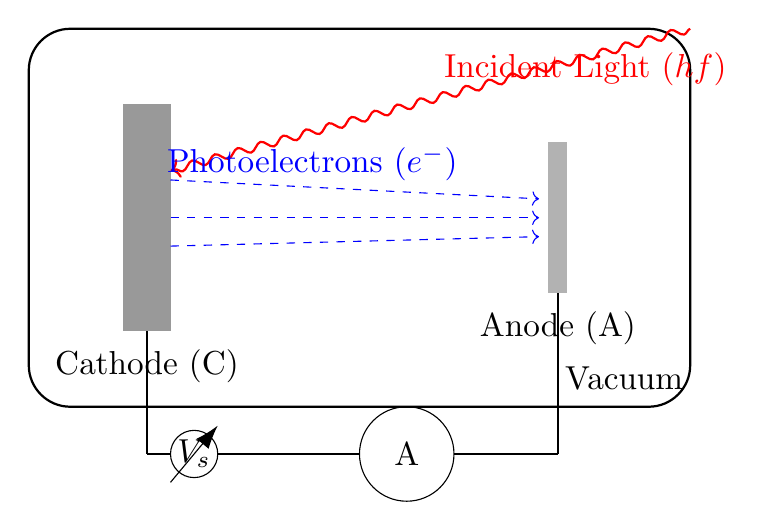
\begin{tikzpicture}[scale=1.2, every node/.style={transform shape}]
    % Vacuum Tube
    \draw[thick, rounded corners=15pt] (-3.5,-2) rectangle (3.5,2);
    \node at (2.8, -1.7) {Vacuum};
    
    % Electrodes
    \fill[gray!80] (-2.5, -1.2) rectangle (-2, 1.2);
    \node[below=2pt of {-2.25, -1.2}] (cathode) {Cathode (C)};
    
    \fill[gray!60] (2, -0.8) rectangle (2.2, 0.8);
    \node[below=2pt of {2.1, -0.8}] (anode) {Anode (A)};
    
    % Incident Light (from top right, hitting cathode)
    \draw[->, decorate, decoration={snake, amplitude=0.5mm, segment length=3mm}, red, thick] (3.5, 2.0) -- (-2.0, 0.5); % Changed start and end points
    \node[above right=1pt of {0.75, 1.25}, red] {Incident Light ($hf$)}; % Adjusted text position

    % Emitted Electrons (from cathode to anode)
    \draw[->, blue, dashed] (-2, 0.4) -- (1.9, 0.2);
    \draw[->, blue, dashed] (-2, 0) -- (1.9, 0);
    \draw[->, blue, dashed] (-2, -0.3) -- (1.9, -0.2);
    \node[above=2pt of {-0.5, 0.2}, blue] {Photoelectrons ($e^-$)};
    
    % External Circuit
    \draw[thick] (-2.25, -1.2) -- (-2.25, -2.5);
    \draw[thick] (2.1, -0.8) -- (2.1, -2.5);
    
    % Ammeter
    \draw[thick] (2.1, -2.5) -- (1, -2.5);
    \draw (0.5, -2.5) circle (0.5cm);
    \node at (0.5, -2.5) {A};
    \draw[thick] (0, -2.5) -- (-1, -2.5);
    
    % Variable Voltage Source
    \draw[thick] (-1, -2.5) -- (-1.5, -2.5);
    \draw (-1.75, -2.5) circle (0.25cm);
    \node at (-1.75, -2.5) {$V_s$};
    \draw[-{Latex[length=3mm, width=2mm]}] (-2, -2.8) -- (-1.5, -2.2);
    \draw[thick] (-2, -2.5) -- (-2.25, -2.5);

\end{tikzpicture}
\captionof{figure}{Schematic of the photoelectric effect experiment.}
\end{center}

\begin{itemize}
    \item \textbf{Work Function ($\phi$):} The minimum energy required to remove an electron from the surface of a material. This is a characteristic property of the material.

    \item \textbf{Einstein's Photoelectric Equation:} This equation is a statement of energy conservation. The energy of an incoming photon is used to overcome the work function, and any remaining energy becomes the kinetic energy of the photoelectron.
    $$ K_{max} = hf - \phi $$
    
    \item \textbf{Stopping Potential ($V_s$):} The minimum reverse potential difference that must be applied to stop the most energetic photoelectrons from reaching the anode. It provides a direct measure of the maximum kinetic energy.
    $$ K_{max} = eV_s $$
    where $e$ is the elementary charge ($1.60 \times 10^{-19} \text{ C}$).
\end{itemize}

\subsection{Radiation Pressure}
Since photons carry momentum, a beam of light exerts a force, and thus a pressure, on any surface it strikes. The magnitude depends on whether the photons are absorbed or reflected.
\begin{itemize}
    \item \textbf{Force ($F$):} Force is the rate of change of momentum, $F = \frac{\Delta p}{\Delta t}$.
    \item \textbf{Pressure ($P_{rad}$):} Pressure is force per unit area, $P_{rad} = \frac{F}{A}$.
\end{itemize}

Two key cases for normal incidence:
\begin{enumerate}
    \item \textbf{Perfect Absorption (Black Surface):} The photon's momentum is completely transferred to the surface. The change in momentum is $\Delta p = p$.
    $$ F = \frac{\text{Total Power}}{c} \quad \text{and} \quad P_{rad} = \frac{I}{c} $$

    \item \textbf{Perfect Reflection (Mirror Surface):} The photon bounces back, so its momentum changes from $p$ to $-p$. The change in momentum is $\Delta p = p - (-p) = 2p$.
    $$ F = \frac{2 \times \text{Total Power}}{c} \quad \text{and} \quad P_{rad} = \frac{2I}{c} $$
\end{enumerate}

\sectionbreak
% ===================================================================
% --- PROBLEM SOLVING ---
% ===================================================================
\section{Guided Problem Solving}

\subsection{Problem 1: SPhO 2023}

\begin{problembox}{Question}
A beam of monochromatic UV light with wavelength 50 nm is incident onto a blackened flat plate of total area 200 cm$^2$. The direction of the beam is normal to the surface of the plate. The beam has an intensity of 24 W m$^{-2}$. Calculate the force exerted by the light beam on the surface of the plate. State any assumption you make in your calculation.
\end{problembox}

\paragraph{Explanation} The term ``blackened flat plate'' implies that the surface is a perfect absorber. The force exerted by the light is the rate at which momentum is transferred. For a perfect absorber, the force is the total power incident on the plate divided by the speed of light.

\paragraph{Solution}
\begin{enumerate}
    \item First, convert the area to SI units.
    $$ A = 200 \text{ cm}^2 = 200 \times (10^{-2} \text{ m})^2 = 0.02 \text{ m}^2 $$
    
    \item Calculate the total power ($P_{tot}$) incident on the plate using the given intensity ($I$).
    $$ P_{tot} = I \times A = (24 \text{ W m}^{-2}) \times (0.02 \text{ m}^2) = 0.48 \text{ W} $$
    
    \item For a perfectly absorbing surface, the force ($F$) is given by:
    $$ F = \frac{P_{tot}}{c} = \frac{0.48 \text{ W}}{3.00 \times 10^8 \text{ m s}^{-1}} = 1.6 \times 10^{-9} \text{ N} $$
    
    \item \textbf{Assumption:} The key assumption made is that the \textbf{``blackened'' plate acts as a perfect absorber}, meaning it absorbs 100\% of the incident photons and reflects none.
\end{enumerate}

\subsection{Problem 2: SPhO 2019}
\begin{problembox}{Question}
A beam of monochromatic light of intensity 50 W m$^{-2}$ is incident normally onto a perfectly reflecting surface. Determine the pressure exerted on that surface by the incident radiation.
\end{problembox}

\paragraph{Explanation} The problem explicitly states the surface is ``perfectly reflecting.'' In this case, the change in momentum for each photon is double that of an absorbed photon. We can directly apply the formula for radiation pressure on a perfectly reflecting surface.

\paragraph{Solution}
\begin{enumerate}
    \item For a perfectly reflecting surface with light at normal incidence, the radiation pressure ($P_{rad}$) is given by:
    $$ P_{rad} = \frac{2I}{c} $$
    
    \item Substitute the given values for intensity ($I$) and the speed of light ($c$).
    $$ P_{rad} = \frac{2 \times (50 \text{ W m}^{-2})}{3.00 \times 10^8 \text{ m s}^{-1}} = \frac{100}{3.00 \times 10^8} \text{ Pa} \approx 3.33 \times 10^{-7} \text{ Pa} $$
\end{enumerate}

\sectionbreak

\subsection{Problem 3: SPhO 2022}
\begin{problembox}{Question}
In a photoelectric experiment, monochromatic ultraviolet light of wavelength 60 nm and intensity 0.7 W m$^{-2}$ is incident onto a cathode which has a surface area of 10 cm$^2$. It is found that the photoelectric current decreases to zero when the anode has a negative potential of 4.25 V with respect to the cathode. When the anode is at a positive potential with respect to the cathode, the saturation photoelectric current is 21.7 nA.
\end{problembox}

\paragraph{(a) Calculate the linear momentum of the photoelectrons which are emitted with the maximum kinetic energy.}

\subparagraph{Explanation} The stopping potential ($V_s = 4.25$ V) gives the maximum kinetic energy ($K_{max}$) of the photoelectrons. From $K_{max}$, we can calculate the momentum using the classical kinetic energy formula, $K = p^2 / (2m)$.

\subparagraph{Solution}
\begin{enumerate}
    \item Calculate $K_{max}$ from the stopping potential.
    \begin{align*}
        K_{max} &= eV_s \\
        &= (1.60 \times 10^{-19} \text{ C})(4.25 \text{ V}) \\
        &= 6.80 \times 10^{-19} \text{ J}
    \end{align*}
    
    \item Calculate the momentum ($p_{max}$) using the kinetic energy formula. ($m_e = 9.11 \times 10^{-31}$ kg).
    \begin{align*}
        p_{max} &= \sqrt{2m_e K_{max}} \\
        &= \sqrt{2(9.11 \times 10^{-31} \text{ kg})(6.80 \times 10^{-19} \text{ J})} \\
        &= \sqrt{1.238 \times 10^{-48} \text{ kg}^2 \text{m}^2 \text{s}^{-2}} \\
        &\approx 1.11 \times 10^{-24} \text{ kg m s}^{-1}
    \end{align*}
\end{enumerate}

\paragraph{(b) What is the ratio of $\frac{N_{e}}{N_{p}}$ where $N_{e}$ \& $N_{p}$ are the rate of emission of photoelectrons and number of photon incident onto the cathode per second?}

\subparagraph{Explanation} The rate of photoelectron emission ($N_e$) is found from the saturation current ($I_{sat}$). The rate of incident photons ($N_p$) is found by calculating the total power on the cathode and dividing by the energy of a single photon. The ratio $\frac{N_e}{N_p}$ is the quantum efficiency.

\subparagraph{Solution}
\begin{enumerate}
    \item Find the rate of electron emission ($N_e$) from the saturation current, $I_{sat} = 21.7 \text{ nA} = 21.7 \times 10^{-9}$ A.
    $$ N_e = \frac{I_{sat}}{e} = \frac{21.7 \times 10^{-9} \text{ A}}{1.60 \times 10^{-19} \text{ C}} \approx 1.356 \times 10^{11} \text{ s}^{-1} $$
    
    \item Find the energy of a single photon ($E_p$) with $\lambda = 60$ nm.
    $$ E_p = \frac{hc}{\lambda} = \frac{(6.63 \times 10^{-34} \text{ J s})(3.00 \times 10^8 \text{ m s}^{-1})}{60 \times 10^{-9} \text{ m}} \approx 3.315 \times 10^{-18} \text{ J} $$
    
    \item Find the total power ($P_{tot}$) incident on the cathode area, $A = 10 \text{ cm}^2 = 1.0 \times 10^{-3} \text{ m}^2$.
    $$ P_{tot} = I \times A = (0.7 \text{ W m}^{-2})(1.0 \times 10^{-3} \text{ m}^2) = 7.0 \times 10^{-4} \text{ W} $$
    
    \item Find the rate of photon incidence ($N_p$).
    $$ N_p = \frac{P_{tot}}{E_p} = \frac{7.0 \times 10^{-4} \text{ W}}{3.315 \times 10^{-18} \text{ J}} \approx 2.112 \times 10^{14} \text{ s}^{-1} $$
    
    \item Calculate the final ratio.
    $$ \frac{N_e}{N_p} = \frac{1.356 \times 10^{11}}{2.112 \times 10^{14}} \approx 6.42 \times 10^{-4} $$
\end{enumerate}

\paragraph{(c) One of the electrons with maximum kinetic energy makes a collision with a hydrogen atom which is in the ground state. What are the possible wavelengths of the photon emitted when the hydrogen atom de-excites?}

\subparagraph{Explanation} We must first determine if the colliding electron has enough energy to excite the hydrogen atom from its ground state ($n=1$) to any higher energy level. The energy levels of hydrogen are given by $E_n = -13.6/n^2$ eV. The minimum energy for excitation is the difference between the first excited state ($n=2$) and the ground state.

\subparagraph{Solution}
\begin{enumerate}
    \item Convert the electron's maximum kinetic energy to electron-volts (eV).
    $$ K_{max} = \frac{6.80 \times 10^{-19} \text{ J}}{1.60 \times 10^{-19} \text{ J/eV}} = 4.25 \text{ eV} $$
    
    \item Calculate the energy of the hydrogen atom's ground state ($n=1$) and first excited state ($n=2$).
    \begin{align*}
        E_1 &= -\frac{13.6}{1^2} \text{ eV} = -13.6 \text{ eV} \\
        E_2 &= -\frac{13.6}{2^2} \text{ eV} = -3.4 \text{ eV}
    \end{align*}
    
    \item Calculate the minimum energy ($\Delta E_{1\to2}$) required to excite the atom.
    $$ \Delta E_{1\to2} = E_2 - E_1 = (-3.4 \text{ eV}) - (-13.6 \text{ eV}) = 10.2 \text{ eV} $$
    
    \begin{center}
    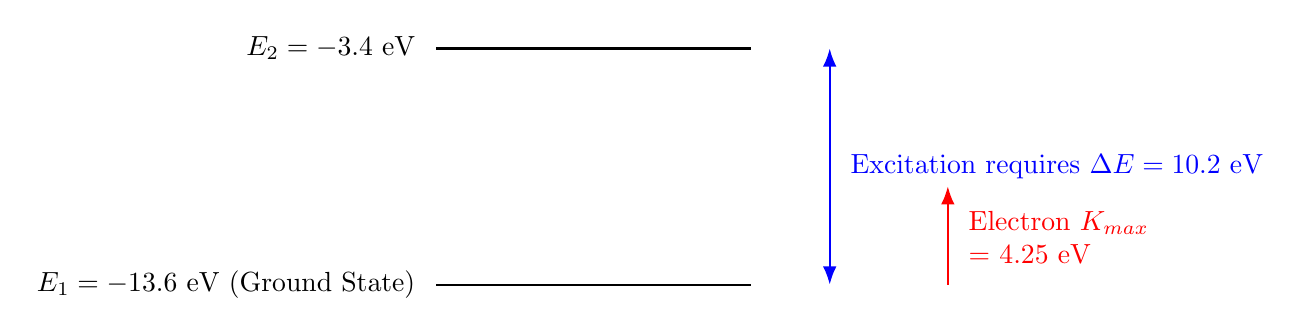
\begin{tikzpicture}
        % Energy Levels
        \draw[thick] (0,0) -- (4,0);
        \node[left=4pt] at (0,0) {$E_1 = -13.6$ eV (Ground State)};
        \draw[thick] (0,3) -- (4,3);
        \node[left=4pt] at (0,3) {$E_2 = -3.4$ eV};
        
        % Excitation Arrow
        \draw[<->, >=Latex, thick, blue] (5,0) -- (5,3);
        \node[right=4pt, blue] at (5,1.5) {Excitation requires $\Delta E = 10.2$ eV};
        
        % Electron Energy Arrow
        \draw[->, >=Latex, thick, red] (6.5,0) -- (6.5,1.25);
        \node[right=4pt, red, align=left] at (6.5,0.6) {Electron $K_{max}$ \\ = $4.25$ eV};
    \end{tikzpicture}
    \end{center}
    
    \item \textbf{Conclusion:} The incident electron's kinetic energy ($4.25$ eV) is less than the minimum energy required to excite the hydrogen atom ($10.2$ eV). Therefore, the collision is elastic, and the hydrogen atom remains in its ground state.
    
    \item Since the atom is not excited, it cannot de-excite by emitting a photon. Thus, \textbf{no photons are emitted}.
\end{enumerate}

\end{document}
% ===================================================================
% --- DOCUMENT END ---
% ===================================================================